\section{Dexterity Network}
\seclabel{dexnet}

%\TODO{Perhaps a cleaner transition here}
We now extend robust grasp planning to leverage prior data from a set of objects by introducing the Dexterity Network (Dex-Net) 1.0, a growing dataset of over 10,000 prior 3D object models annotated with parallel-jaw grasps and a similarity metric to efficiently index objects.
The dataset is selected to represent objects that might be encountered in warehousing or the home such as containers, tools, tableware, and toys.
%Laser-scanned models from the KIT object database~\cite{kasper2012kit}, the Amazon Picking Challenge objects, BigBIRD~\cite{singh2014bigbird}, and YCB ~\cite{calli2015benchmarking} constitute 355 of the total models.
%The majority of Dex-Net is synthetic 3D mesh models from 3DNet\cite{wohlkinger20123dnet}, a benchmark for object detection in robotics research,  ModelNet~\cite{wu20143d}, a benchmark for 3D model classification, and the SHREC 2014 large scale object retrieval challenge~\cite{li2015comparison}, a competition benchmark with many categories to test the state-of-the-art in shape retrieval annually.
\tabref{datasets} details the data sources and their sizes.

{%
\setlength{\tabcolsep}{1pt}

\begin{table}[t]
\centering
        \begin{tabular}{L{2.5cm} || R{1.5cm} | R{1.5cm}}
        \multicolumn{1}{c ||}{\specialcell{\bf Dataset}} & \multicolumn{1}{c |}{\specialcell{\bf \# Models}}  & \multicolumn{1}{c}{\specialcell{\bf Synthetic?}} \\
        \hline & & \\ [-1.5ex]
        SHREC2014~\cite{li2015comparison} & 8,987 & Y\\
        ModelNet40~\cite{wu20153d} & $^*$2,539 & Y \\
        3DNet~\cite{wohlkinger20123dnet} & 1,371 & Y \\
        KIT~\cite{kasper2012kit} & 129 & N \\
        BigBIRD~\cite{singh2014bigbird} & 120 & N \\
        YCB~\cite{calli2015benchmarking} & 80 &  N\\
        APC & 26 & N\\
        \hline & & \\ [-1.5ex]
        {\bf Total} & 13,252 & \\ 
        \end{tabular}
        \caption{The seven datasets used in Dex-Net 1.0 with the number of models in the dataset and whether or not the models were laser-scanned. $^*$ indicates a subset of the original dataset. }
		\tablabel{datasets}
\vspace*{-15pt}
\end{table}
}

%\begin{figure}[t!]
%\centering
%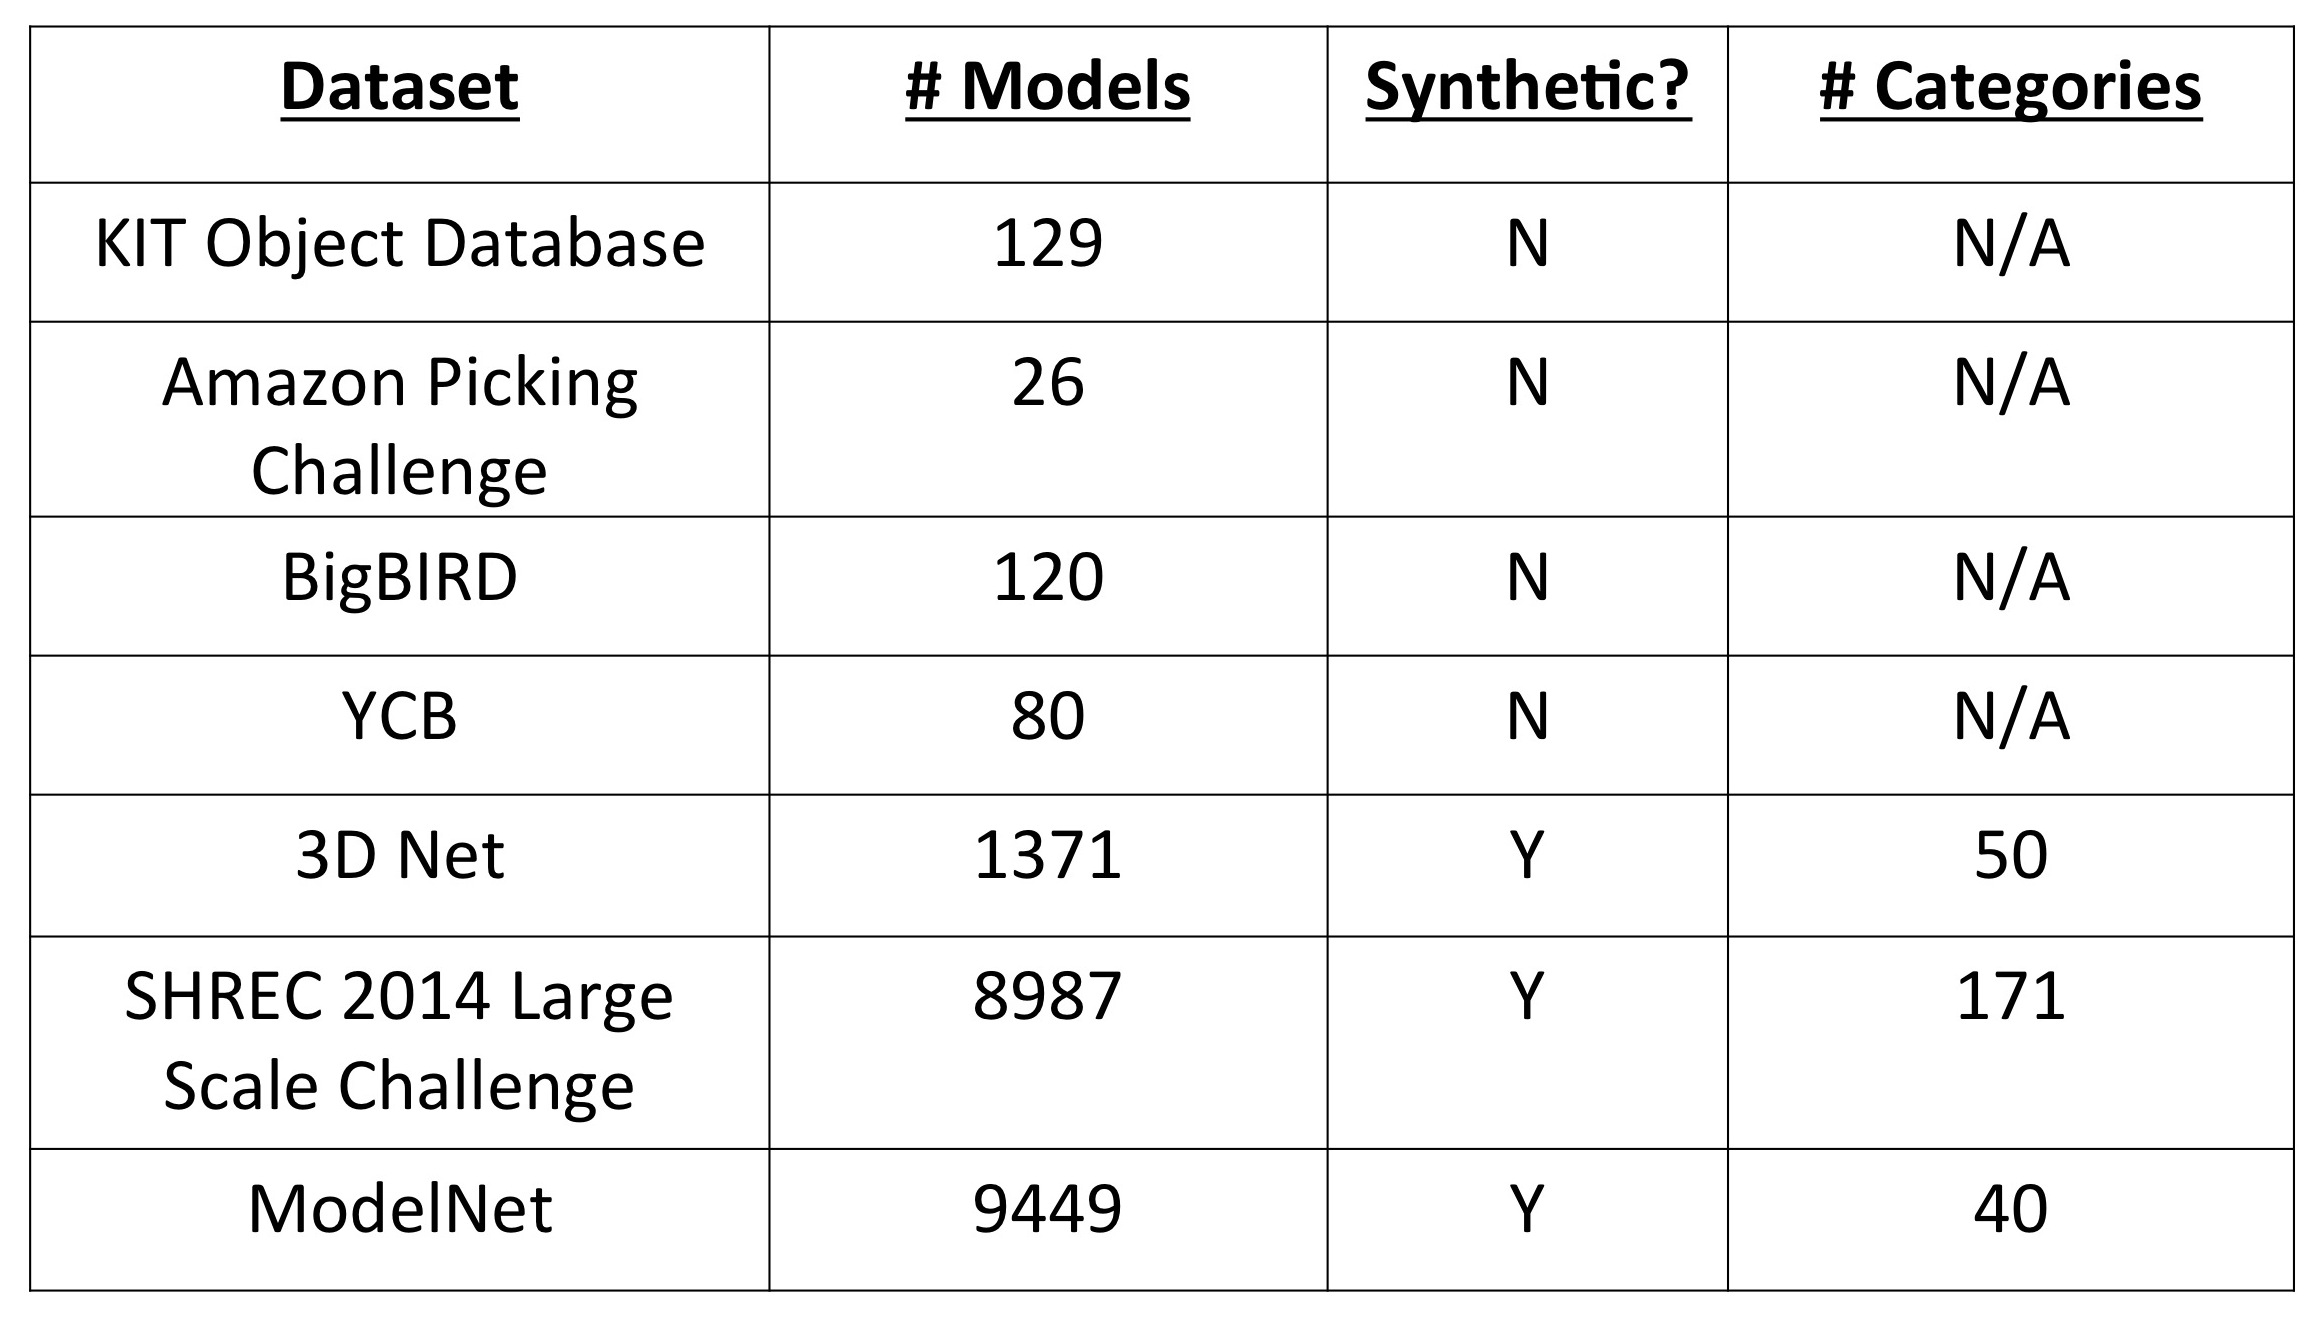
\includegraphics[scale=0.1]{figures/dataset_table.jpg}
%\caption{\TODO{Remove columns}}
%\figlabel{datasets}
%\vspace*{-15pt}
%\end{figure}


\subsection{Data Cleaning}
Each object in Dex-Net is specified as a 3D mesh $\mX = \{\mV, \mT\}$ where $\mV = \{\bv_1, ..., \bv_V\}$ is a set of $V$ vertices such that $\bv_i \in \bR^3$ for $i = 1, ..., V$ and $\mT = \{t_1, ..., t_F\}$  is a set of $F$ triangles such that $t_j \in \mathbb{Z}_{+}^3$ for $j = 1, ..., F$.
We preprocess each model by first removing unreferenced vertices and degenerate triangles.
Next, we compute the object reference frame by performing Principal Component Analysis (PCA) on the vertices of the mesh and aligning the $z$-axis with the first principal component and the $y$-axis with the second principal component
We then set the object center of mass $\bz$ to be the center of the bounding box for the reoriented mesh.
Since synthetic models may not be specified in meters, we also rescale each mesh such that the smallest dimension of the bounding box lies within $w = 0.1m$, which is approximately the maximal opening width of a PR2 gripper.
Finally, we convert each mesh to an SDF using SDFGen~\cite{sdfgen}, an open-source C++ tool.

\subsection{Grasp Sampling}
\seclabel{grasp-sampling}
Each 3D object $\mO_i$ in Dex-Net is labelled with up to 250 parallel-jaw grasps and the $P_F$ for each.
We generate $N_g$ grasps for each object using a modification of the 2D algorithm presented in Smith et al.~\cite{smith1999computing} to concentrate samples on grasps that are antipodal~\cite{mahler2015gp}.
Let $w$ be the maximal opening of the gripper, $\hat{\gamma}$ be a sampled friction coefficient, and $\mS$ be the set of points on the object surface for an SDF $f$ as described in \secref{grasp-param}.
To sample a single grasp, we first generate a contact point $\bc_1$ by sampling uniformly from $\mS$ using rejection sampling.
Next we sample a direction $\bv \in \bS^2$ uniformly at random from the friction cone and compute:
%\vspace{-2ex}
\begin{align*}
	\bc_2 = \bc_1 + (w / 2 - t_2^*) \bv  &&  \bx = 0.5 (\bc_1 + \bc_2)
\end{align*}
\noindent where $t_2^*$ is defined in \secref{contact}.
This yields a grasp $\bg_{i,k} = (\bx, \bv)$.
We add $\bg_{i,k}$ to our candidate set if the contacts are antipodal~\cite{mahler2015gp}, or $\bv^T \bn_1 \leq \cos(\arctan(\hat{\gamma}))$ and $\bv^T \bn_2 \leq \cos(\arctan(\hat{\gamma}))$.

We then evaluate $P_F(\bg)$ using Monte-Carlo integration~\cite{kehoe2012toward} by sampling the object pose, gripper pose, and friction random variables $N_s$ times and recording $S_{i,k}$, the number of samples for which grasp $\bg_{i,k}$ was in force closure.
Formally, our full dataset of $N_o$ 3D objects and $N_g$ grasps per object is $\mD = \{ (S_{i, k}, \mY_{i, k}) \big| i = \{1, ..., N_o\}, k = \{1, ..., N_g\} \}$ where $\mY_{i,k} = (\bg_{i, k}, \mO_i) \in \mM$ is a grasp-object pair in our Grasp Moduli Space.


%We generate a set of grasps for each object in the network using the method of \secref{candidates} and evaluate the probability of force closure for each grasp using brute-force Monte Carlo integration as a benchmark~\cite{kehoe2012toward}.
%As the number of models is quite large, we distribute the grasp labelling for each object across virtual machines in Google Compute Engine and aggregate the results at the end.

\subsection{Grasp Differential Heightmap Features}
\seclabel{grasp-similarity}
To measure grasp similarity, we also embed each parallel-jaw grasp $\bg$ on object $\mO$ in Dex-Net in a feature space based on 2D projections of the local surface orientation, a variant of grasp heightmaps~\cite{herzog2012template, kappler2015leveraging}.
Let $d_h \in \mathbb{Z}$ be a number of pixels for the projection, let $\mP = \{-d_h, ..., d_h\}$ be row / column pixel indices, let $\delta \in \mathbb{R}$ be the pixel resolution in meters, and let $r \in \mathbb{R}$ be a minimum projection distance.
Furthermore, let $\bc_i, i = 1, 2$ be a contact point for grasp $\bg$ and let $\bt_1, \bt_2$ be two orthogonal unit vectors to the grasp approach direction $\bv$.
Our heightmap at contact $i$, $\bh_{i}: \mP \times \mP \rightarrow \bR$, maps discrete locations along the tangent plane specified by $\bt_1, \bt_2$ to the distance to the surface along the grasp axis $\bv$.
To compute the heightmap value at pixel $u,v \in \mP$, we first compute the 3D location of the pixel on the plane $\bp_i(u,v) = \bc_i + \delta u \bt_1 + \delta v \bt_2$.
Then we assign
\begin{align*}
	\bh_i(u,v) = \minimum{t \geq -r} t \text{ such that } f\left( \bp_i(u,v) + (-1)^{i} \bv \right) = 0
\end{align*}
\noindent where $f$ is the SDF of object $\mO$. 
We then make $\bh_i$ rotation-invariant by orienting its axes to align with the eigenvectors of the weighted covariance matrix of the 3D surface points that generate the heightmap as described in~\cite{tombariunique}.
\figref{local-feature-model} illustrates local surface patches extracted by this procedure.
Since force closure depends largely on object surface normals at the contact points, we finally take the $x$- and $y$-image gradients of $\bh_i$ to form differential heightmaps $\bd_{i,x}$ and $\bd_{i,y}$.
Our full feature vector for the grasp-object pair is $\eta(\bg, \mO) = (\bd_{1,x}, \bd_{1,y}, \bd_{2,x}, \bd_{2,y})$, which we store for each grasp in Dex-Net.

\begin{figure}[t!]
\centering
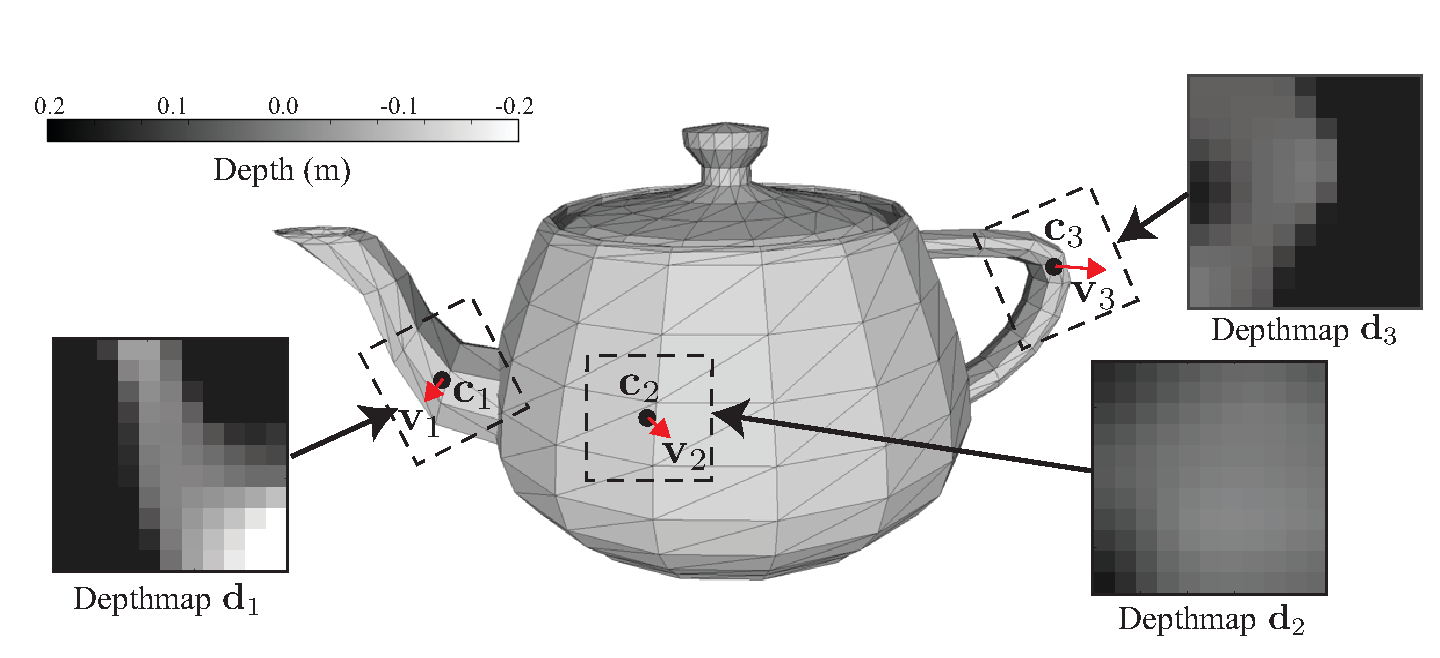
\includegraphics[scale=0.325]{figures/illustrations/local_feature_model.eps}
\caption{Illustration of three local surface heightmaps extracted on a teapot. Each heightmap is ``rendered" along the grasp axis at each contact point and oriented by the local directions of maximum variation in the heightmap.  We extract the gradients of these heightmaps to measure similiarity between grasps in Dex-Net.}
\figlabel{local-feature-model}
\vspace*{-15pt}
\end{figure}

\section{Deep Learning for Object Similarity}
\seclabel{object-similarity}
In order to efficiently index prior 3D object and grasp data from Dex-Net, we embed each object in a Euclidean vector space in which similar objects will be close together.
We use multi-view Convolutional Neural Networks (MV-CNNs)~\cite{aubry2015understanding, su2015multi}, a new method for 3D shape classification that outperforms the accuracy of previous methods by over 10\% on the ModelNet40 shape classification benchmark and uses the powerful features learned by CNNs on millions of images~\cite{krizhevsky2012imagenet}.
 
\figref{global-feature-model} illustrates the approach.
Let $R$ be the maximum dimension of the object bounding box.
We first render every object on a white background in a total of $N_c = 50$ virtual camera views oriented toward the object center and discretized on a viewing sphere along angle increments $\delta_{\theta} = \frac{4 \pi}{N_c}$ and $\delta_{\phi} = \frac{2 \pi}{N_c}$ and radii $r = R, 2R$.
Then we train a CNN with the architecture of AlexNet~\cite{krizhevsky2012imagenet} to predict the 3D object class label for the rendered images on a training set of models. 
We initialize the weights of our network with the weights learned on ImageNet by Krizhevsky et al.~\cite{krizhevsky2012imagenet} and optimize using Stochastic Gradient Descent (SGD). 
Next, we pass each of the $N_c$ views of each object through the optimized CNN and max-pool the output of the fc7 layer, the highest layer of the network before the class label prediction. 
Finally, we use Principal Component Analysis (PCA) to reduce the max-pooled output from 4028 dimensions to 100 dimensions.
This yields our representation $\psi(\mO) \in \mathbb{R}^{100}$ for each object.
%Our method differs from the MV-CNN of Su et al.~\cite{su2015multi} because we use PCA for the final output, while Su et al. use a second CNN on the output of the pooled views. 

Given the MV-CNN object representation, we measure the dissimilarity between two objects $\mO_i$ and $\mO_j$ by the Euclidean distance $\| \psi(\mO_i) - \psi(\mO_j) \|_2$.
For efficient lookups of similar objects, Dex-Net contains a KD-Tree nearest neighbor query structure with the feature vectors of all prior objects.

In our implementation, we trained our MV-CNN using the Caffe library~\cite{jia2014caffe} on rendered images from a training set of approximately $6,000$ 3D models from the SHREC 2014 dataset ~\cite{li2015comparison} for 500,000 iterations of SGD.
The final PCA step captured approximately 85\% of the variance of the vectors.
The image classification training step had a test accuracy of 76\%.
To validate our implementation, we tested our method on the SHREC 2014 challenge dataset and achieved a 1-NN accuracy of 86.7\%, compared to 86.8\% achieved by the winner of SHREC 2014~\cite{li2015comparison}.

\begin{figure}[t!]
\centering
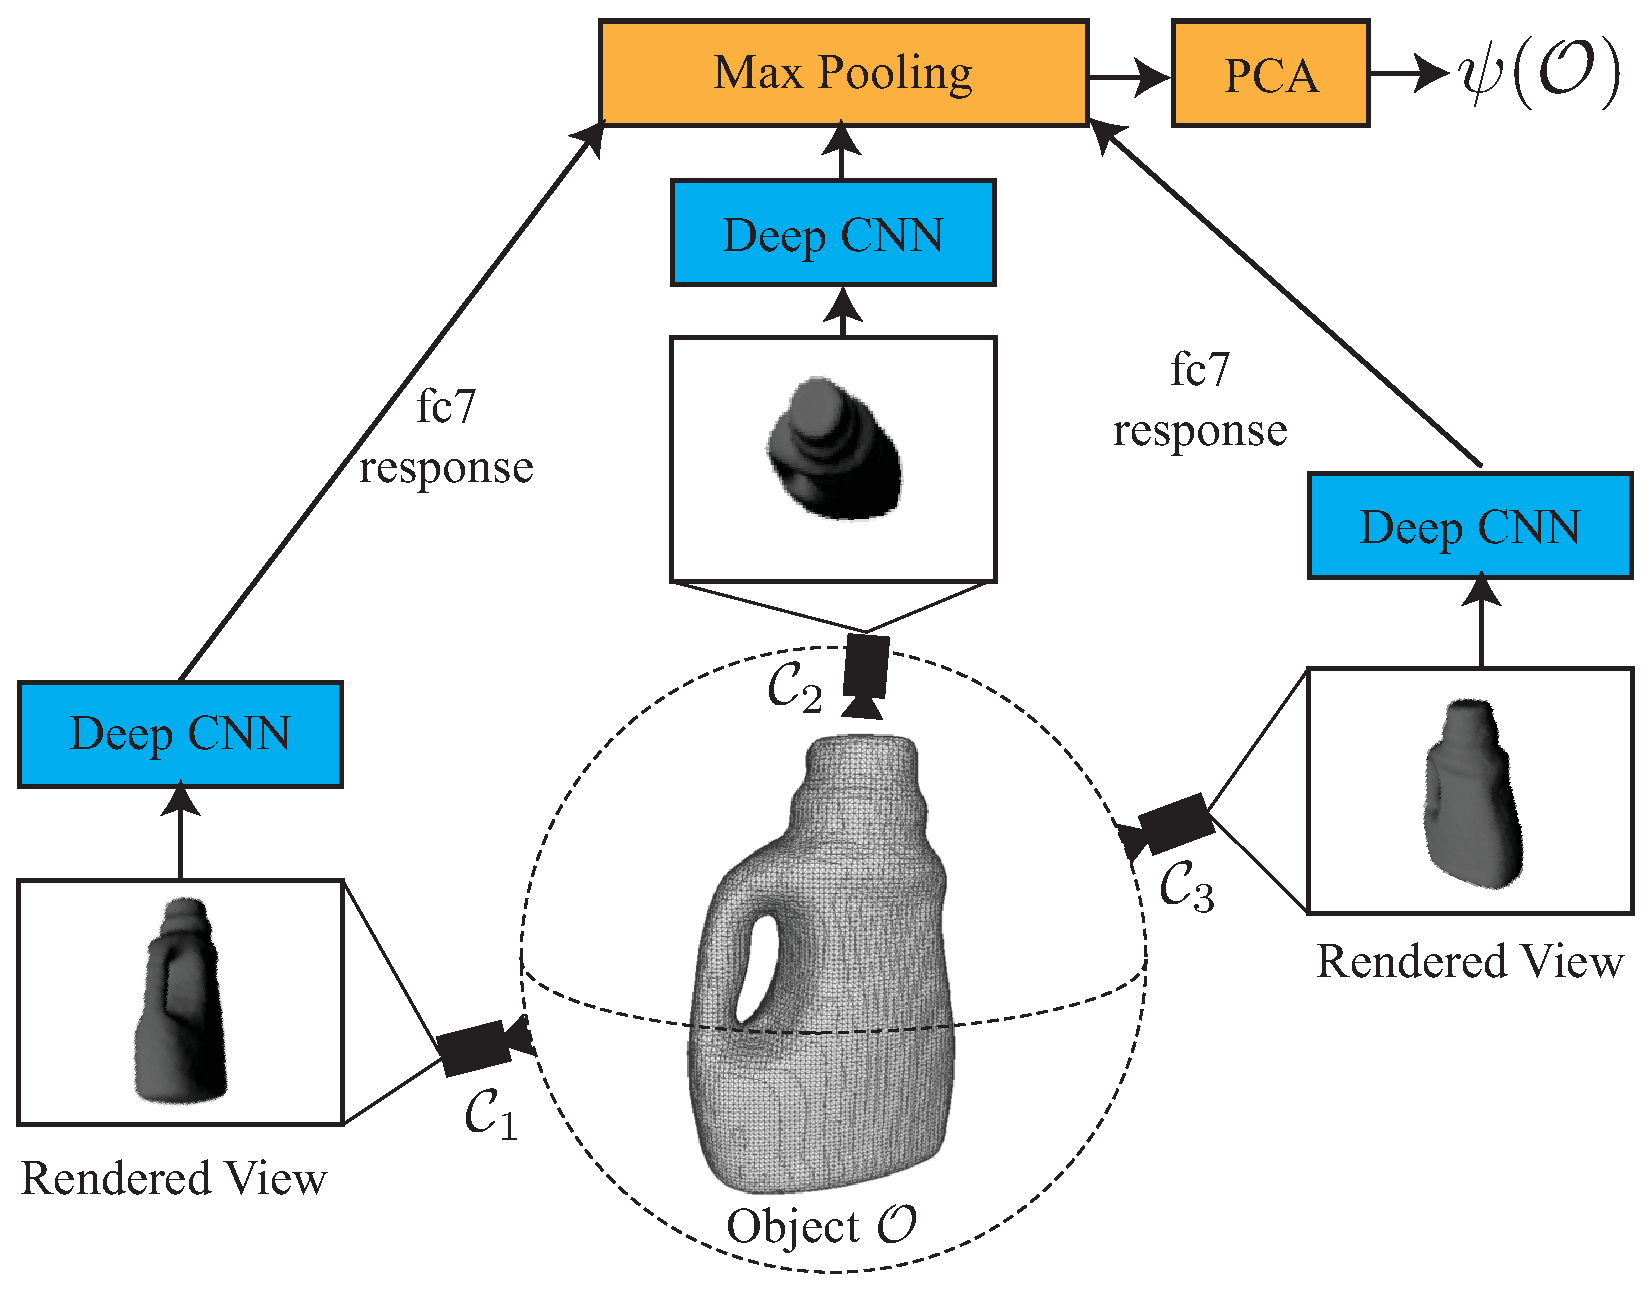
\includegraphics[scale=0.25]{figures/illustrations/cnn_model.eps}
\caption{Illustration of our method for embedding 3D object models in a Euclidean vector space for computing global shape similiarty. We pass a set of 50 virtually rendered camera viewpoints discretized around a sphere through a deep Convolutional Neural Network (CNN) with the AlexNet~\cite{krizhevsky2012imagenet} architecture. Finally, we take the maximum fc7 response across each of the 50 views for each dimension and run PCA to reduce the dimensionality of the output.}
\figlabel{global-feature-model}
\vspace*{-15pt}
\end{figure}

